%!TEX root = ../template.tex
%%%%%%%%%%%%%%%%%%%%%%%%%%%%%%%%%%%%%%%%%%%%%%%%%%%%%%%%%%%%%%%%%%%%
%% appendix1.tex
%% NOVA thesis document file
%%
%% Chapter with example of appendix with a short dummy text
%%%%%%%%%%%%%%%%%%%%%%%%%%%%%%%%%%%%%%%%%%%%%%%%%%%%%%%%%%%%%%%%%%%%

\typeout{NT FILE appendix1.tex}%

\chapter{Meta-modelo}
\label{app:meta_modelo_app}

\begin{figure}[htbp]
  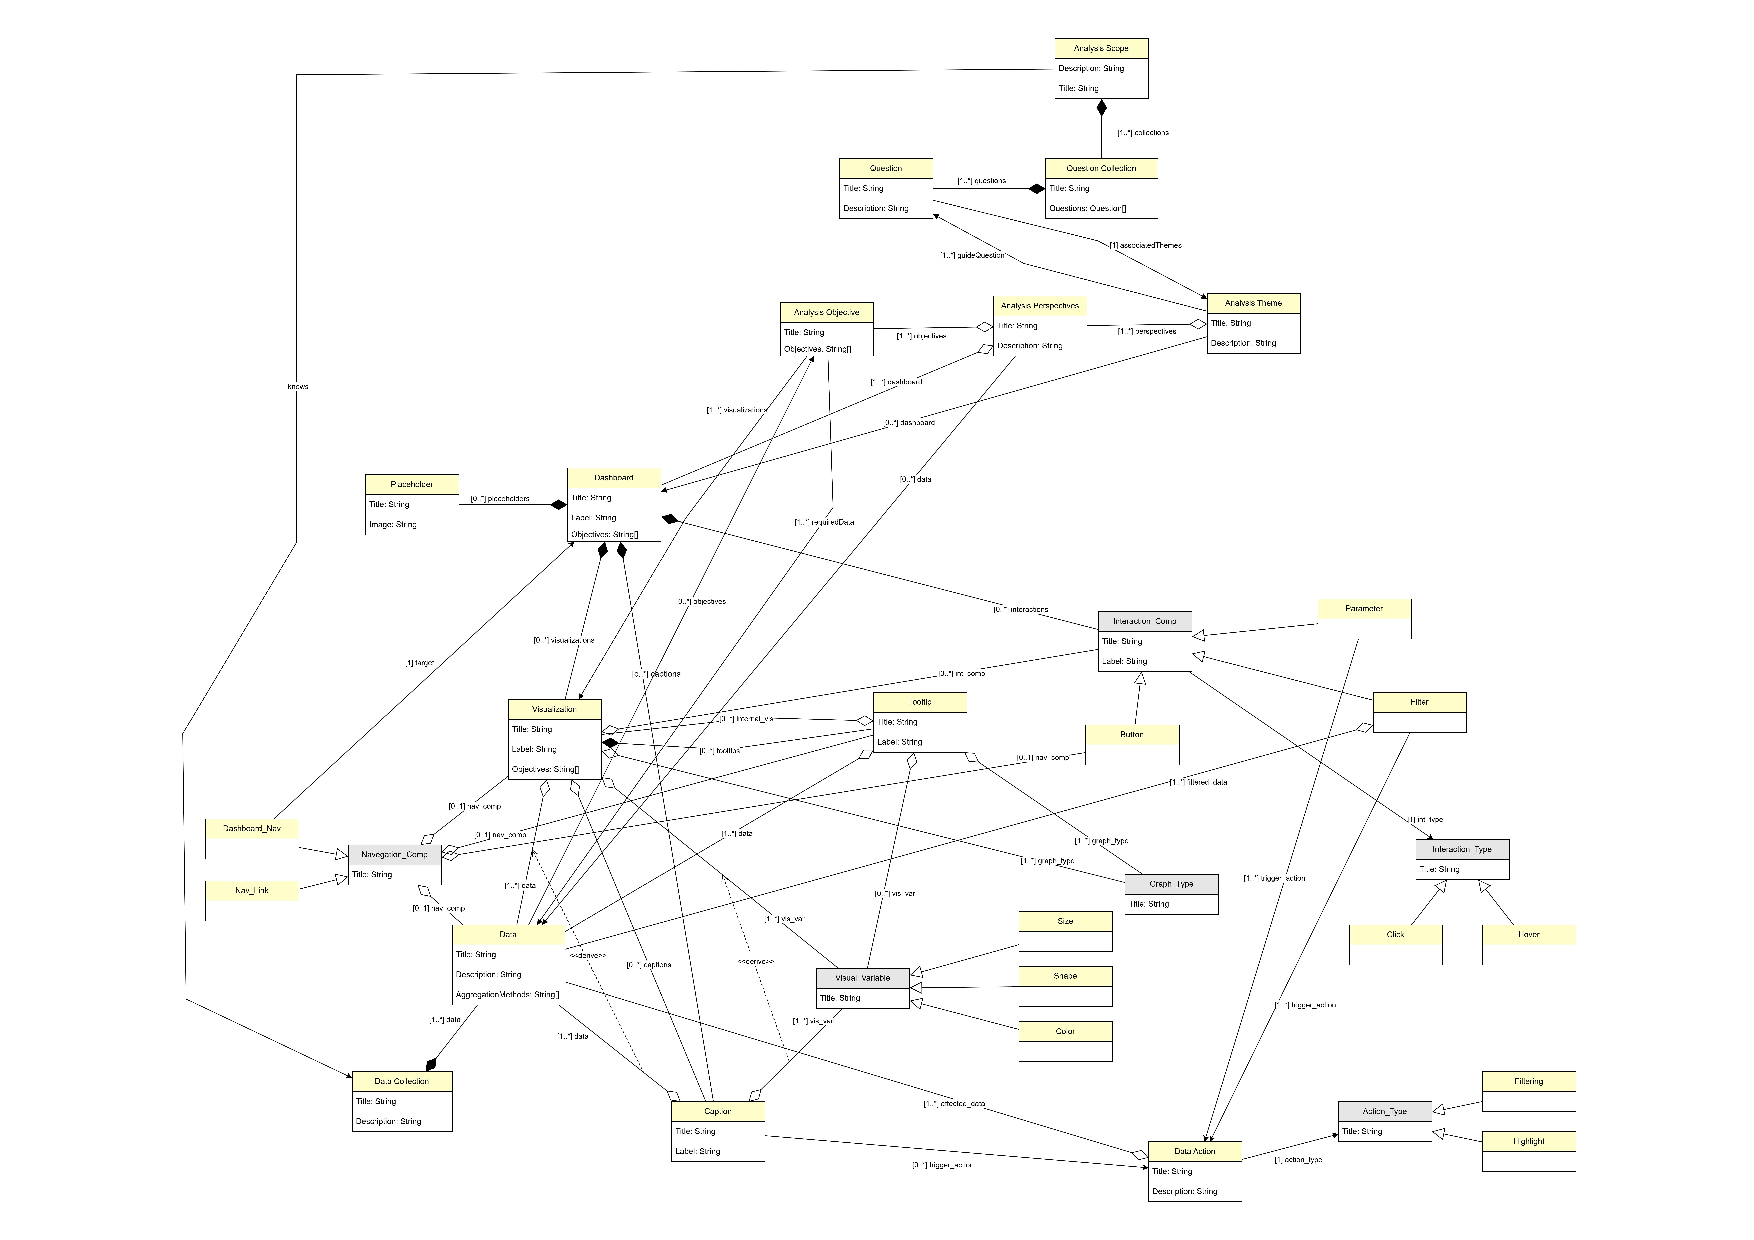
\includegraphics[width=\textwidth, height=4in]{meta_modelo/completeDiagramPDF}
  \caption{Meta-modelo completo.}
  \label{fig:meta_modelo_img}
\end{figure}

\chapter{Protótipo inicial}
\label{app:prototipo_inicial}

\begin{figure}[htbp]
  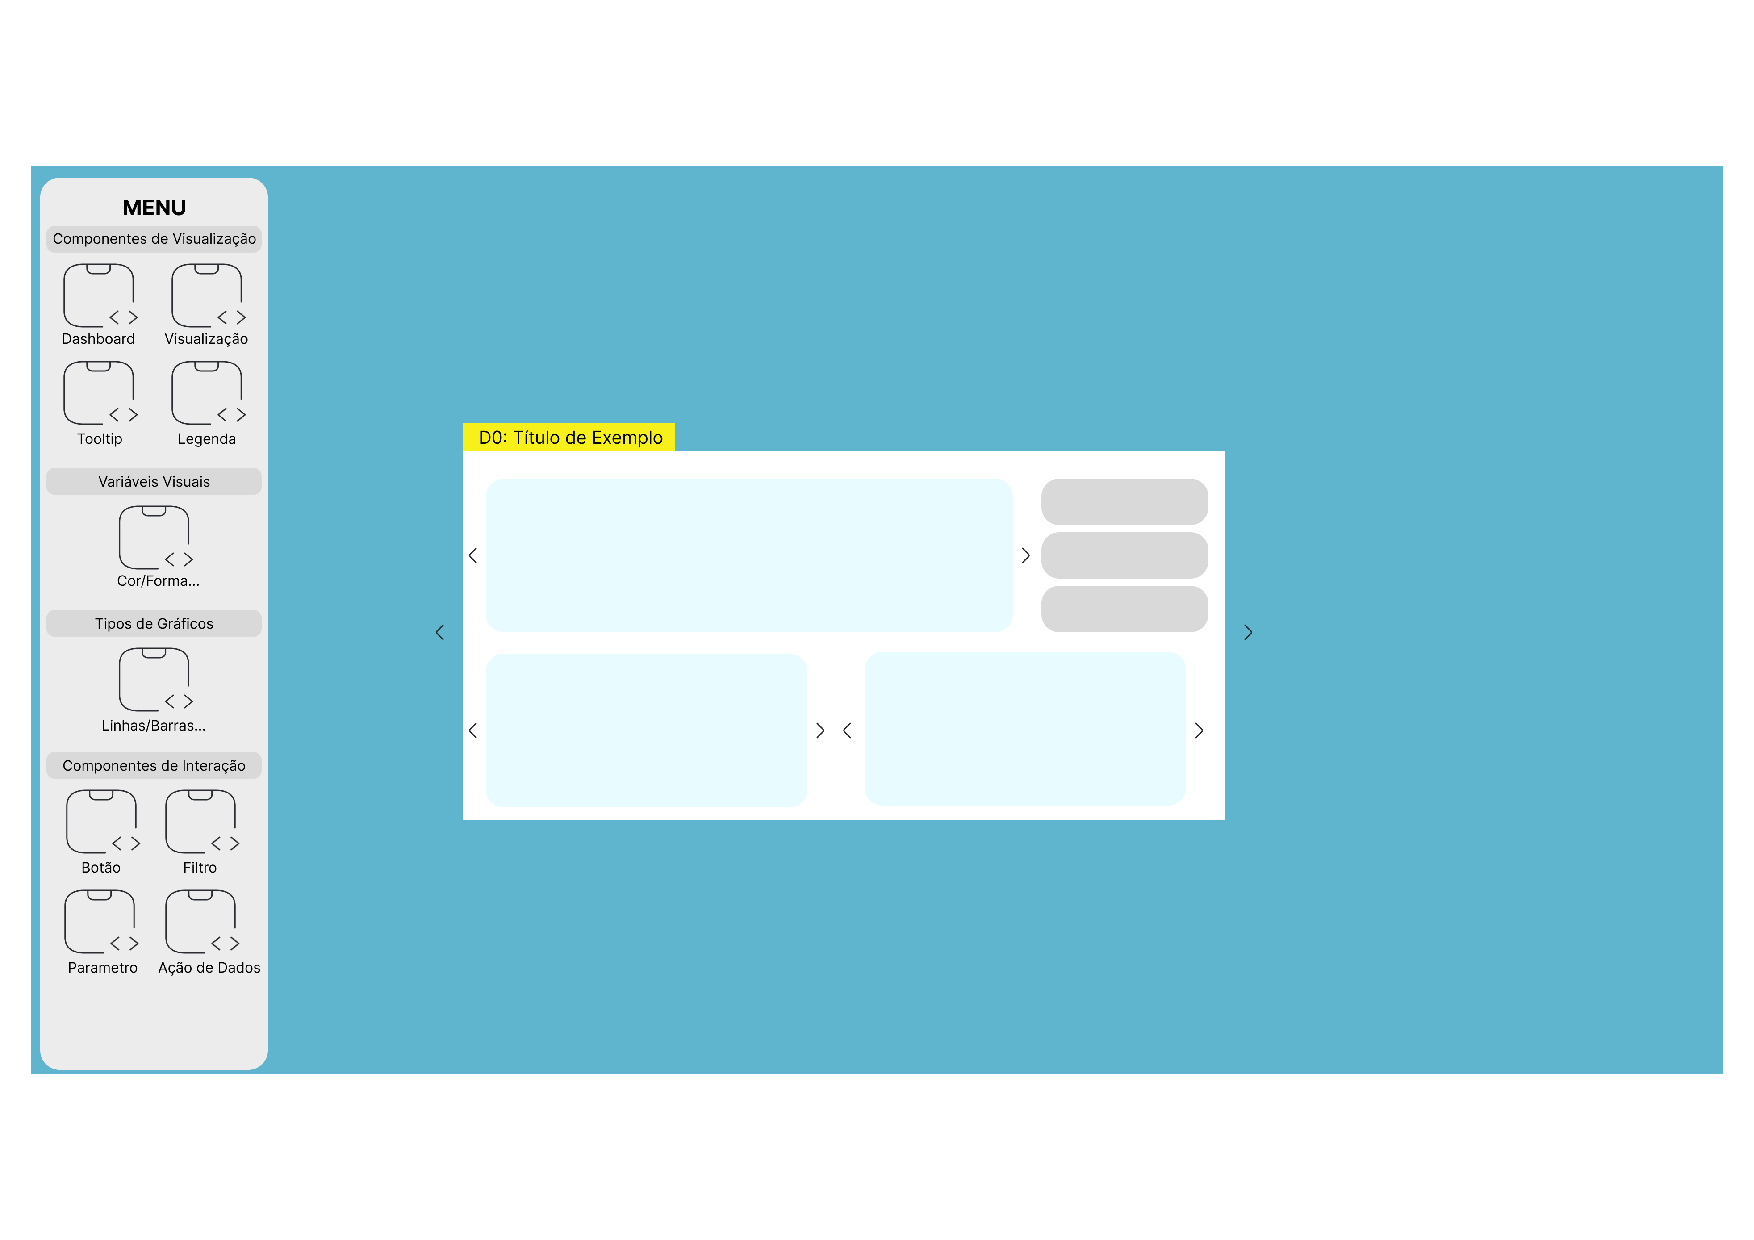
\includegraphics[width=\textwidth, height=4in]{prototipo/prototipo_desktop}
  \caption{Protótipo incial desktop.}
  \label{fig:meta_modelo_img}
\end{figure}

\begin{figure}[htbp]
  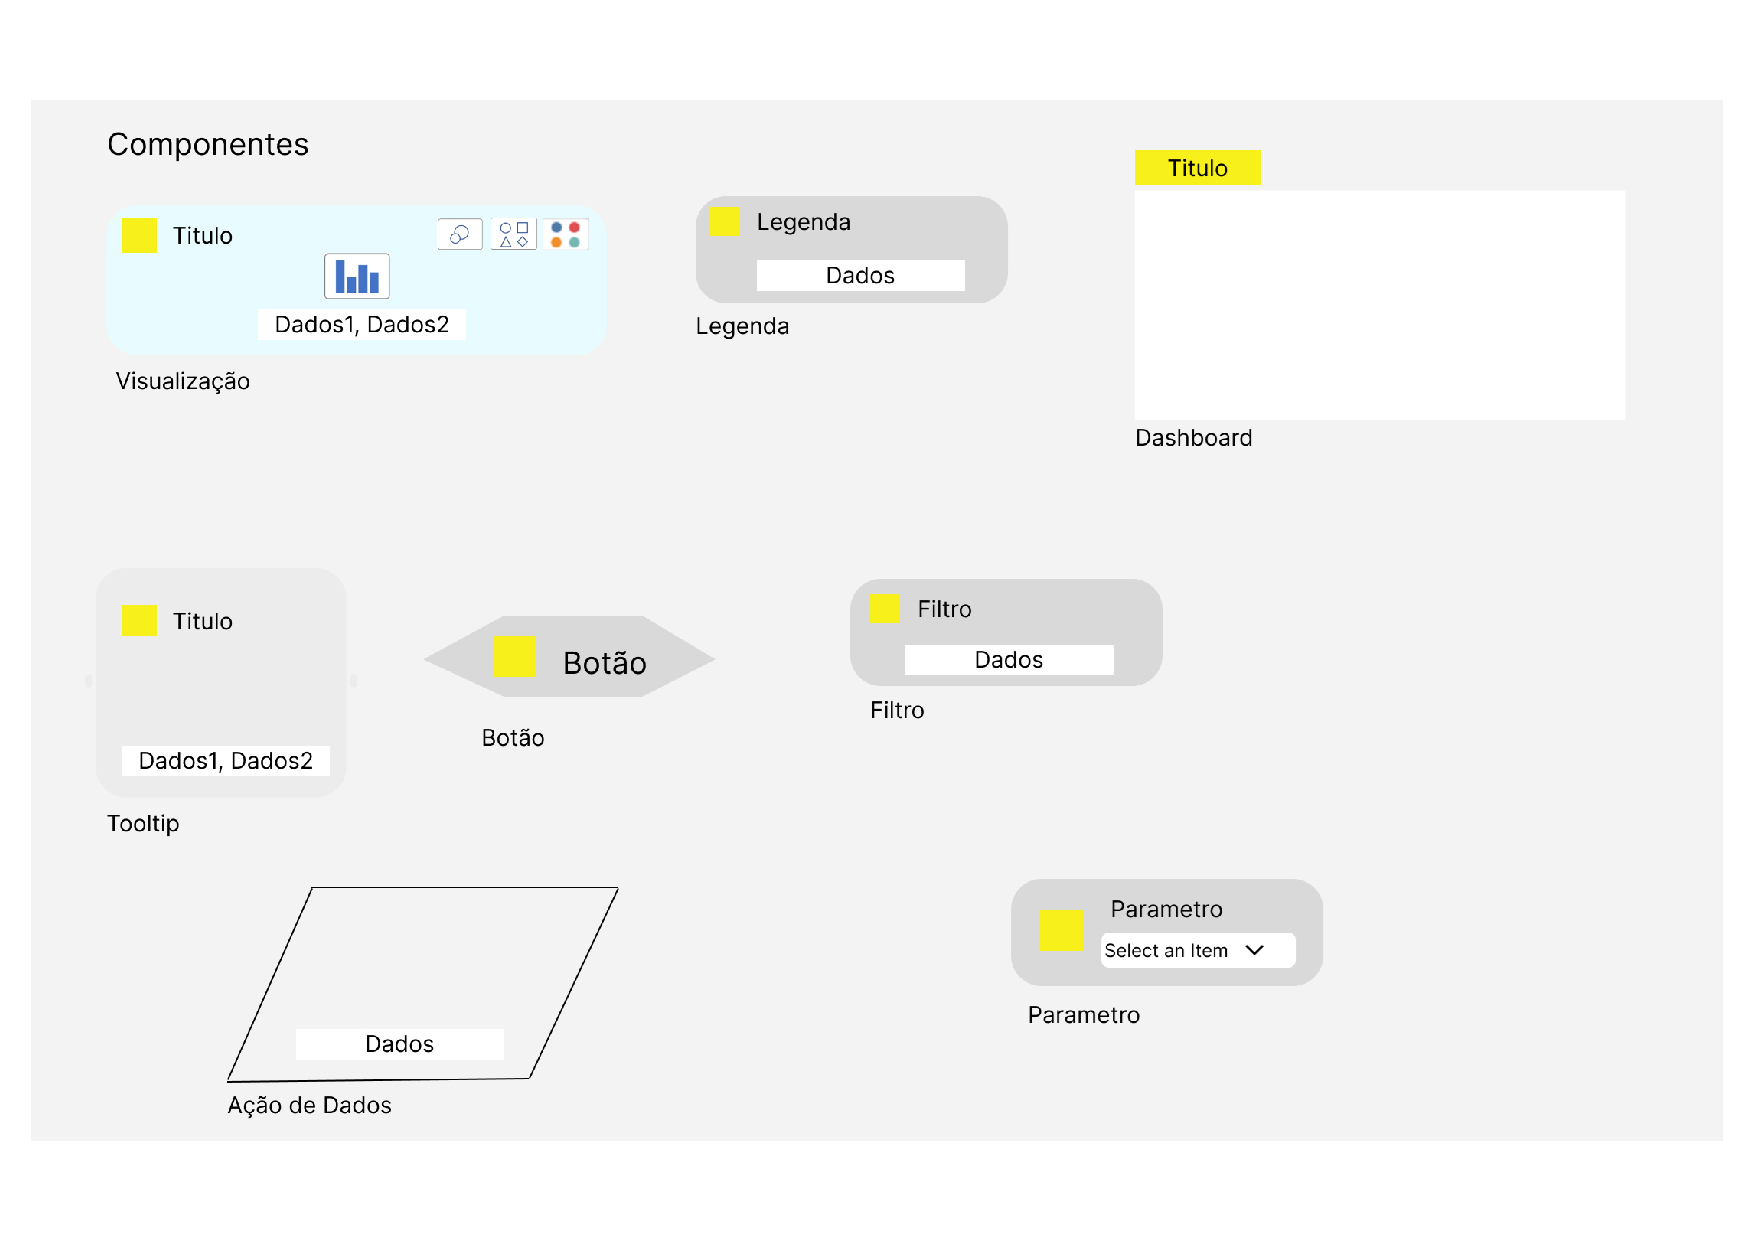
\includegraphics[width=\textwidth, height=4in]{prototipo/prototipo_componentes}
  \caption{Protótipo das componentes. MUDAR PARA A NOVA IMAGEM QUE TENHO PORQUE NESTA O MENU DADOS ESTÁ DESFORMATADO}
  \label{fig:meta_modelo_img}
\end{figure}

\begin{figure}[htbp]
  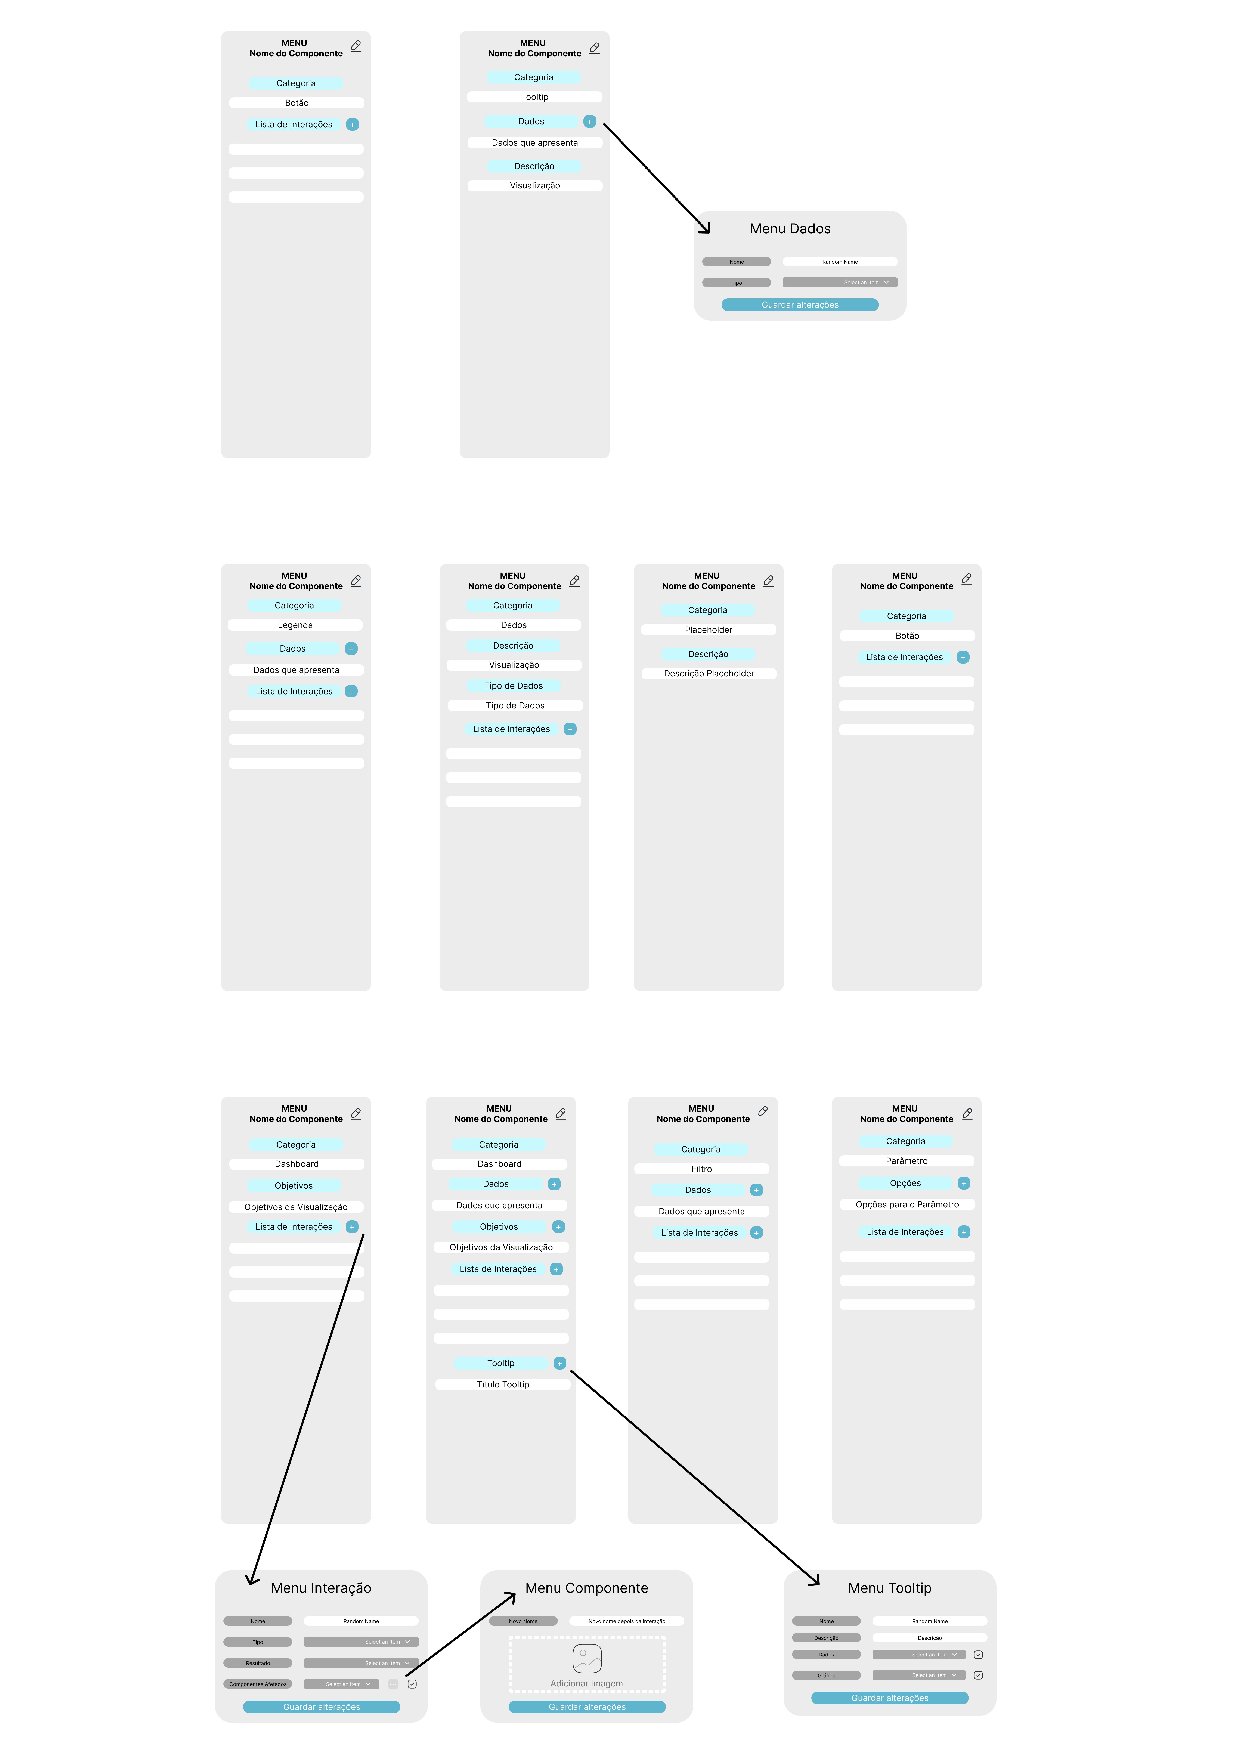
\includegraphics[width=\textwidth, height=4in]{prototipo/prototipo_menus}
  \caption{Protótipo dos menus.}
  \label{fig:meta_modelo_img}
\end{figure}